\documentclass[hidelinks,12pt]{article}
\usepackage[left=0.25cm,top=1cm,right=0.25cm,bottom=1cm]{geometry}
%\usepackage[landscape]{geometry}
\textwidth = 20cm
\hoffset = -1cm
\usepackage[utf8]{inputenc}
\usepackage[spanish,es-tabla]{babel}
\usepackage[autostyle,spanish=mexican]{csquotes}
\usepackage[tbtags]{amsmath}
\usepackage{nccmath}
\usepackage{amsthm}
\usepackage{amssymb}
\usepackage{mathrsfs}
\usepackage{graphicx}
\usepackage{subfig}
\usepackage{standalone}
\usepackage[outdir=./Imagenes/]{epstopdf}
\usepackage{siunitx}
\usepackage{physics}
\usepackage{color}
\usepackage{float}
\usepackage{hyperref}
\usepackage{multicol}
%\usepackage{milista}
\usepackage{anyfontsize}
\usepackage{anysize}
%\usepackage{enumerate}
\usepackage[shortlabels]{enumitem}
\usepackage{capt-of}
\usepackage{bm}
\usepackage{relsize}
\usepackage{placeins}
\usepackage{empheq}
\usepackage{cancel}
\usepackage{wrapfig}
\usepackage[flushleft]{threeparttable}
\usepackage{makecell}
\usepackage{fancyhdr}
\usepackage{tikz}
\usepackage{bigints}
\usepackage{scalerel}
\usepackage{pgfplots}
\usepackage{pdflscape}
\pgfplotsset{compat=1.16}
\spanishdecimal{.}
\renewcommand{\baselinestretch}{1.5} 
\renewcommand\labelenumii{\theenumi.{\arabic{enumii}})}
\newcommand{\ptilde}[1]{\ensuremath{{#1}^{\prime}}}
\newcommand{\stilde}[1]{\ensuremath{{#1}^{\prime \prime}}}
\newcommand{\ttilde}[1]{\ensuremath{{#1}^{\prime \prime \prime}}}
\newcommand{\ntilde}[2]{\ensuremath{{#1}^{(#2)}}}

\newtheorem{defi}{{\it Definición}}[section]
\newtheorem{teo}{{\it Teorema}}[section]
\newtheorem{ejemplo}{{\it Ejemplo}}[section]
\newtheorem{propiedad}{{\it Propiedad}}[section]
\newtheorem{lema}{{\it Lema}}[section]
\newtheorem{cor}{Corolario}
\newtheorem{ejer}{Ejercicio}[section]

\newlist{milista}{enumerate}{2}
\setlist[milista,1]{label=\arabic*)}
\setlist[milista,2]{label=\arabic{milistai}.\arabic*)}
\newlength{\depthofsumsign}
\setlength{\depthofsumsign}{\depthof{$\sum$}}
\newcommand{\nsum}[1][1.4]{% only for \displaystyle
    \mathop{%
        \raisebox
            {-#1\depthofsumsign+1\depthofsumsign}
            {\scalebox
                {#1}
                {$\displaystyle\sum$}%
            }
    }
}
\def\scaleint#1{\vcenter{\hbox{\scaleto[3ex]{\displaystyle\int}{#1}}}}
\def\bs{\mkern-12mu}


%\usepackage{showframe}
\usepackage{apacite}
\title{Funciones de Chebychev \\ \large {Tema 5 - Funciones especiales} \vspace{-3ex}}
\author{M. en C. Gustavo Contreras Mayén}
\date{ }
\begin{document}
\vspace{-4cm}
\maketitle
\fontsize{14}{14}\selectfont
\tableofcontents
\newpage
%Referencia Riley 18.4 Chebyshev functions
\section{Funciones de Chebychev.}
La ecuación diferencial de Chebychev tiene la forma:
\begin{align}
(1 - x^{2}) \, \stilde{y} - x \, \ptilde{y} + \nu^{2} \, y
 = 0
 \label{eq:ecuacion_18_054}
\end{align}
y tiene tres puntos singulares regulares, en $x = -1, 1, \infty$. Al comparar la ecuación con
\begin{align*}
(1 - x^{2}) \, \stilde{y} - x \, \ptilde{y} + \ell (\ell + 1) \, y = 0
\end{align*}
vemos que la ecuación de Chebyshev es muy similar en forma a la ecuación de Legendre. A pesar de esta similitud, la ecuación (\ref{eq:ecuacion_18_054}) no se presenta con mucha frecuencia en problemas físicos, aunque \emph{sus soluciones son de considerable importancia en el análisis numérico}.
\par
El parámetro $\nu$ es un número real dado, pero en casi todas las aplicaciones prácticas toma un valor entero. De aquí en adelante asumimos que $\nu = n$, donde $n$ es un número entero no negativo. Como fue el caso de la ecuación de Legendre, en el uso normal la variable $x$ es el coseno de un ángulo, por lo que $-1 \leq x \leq 1$. Cualquier solución de la ec. (\ref{eq:ecuacion_18_054}) se llama \emph{función de Chebyshev}.
\par
El punto $x = 0$ es un punto ordinario de la ec. (\ref{eq:ecuacion_18_054}), por lo que esperamos encontrar
dos soluciones linealmente independientes de la forma
\begin{align*}
y = \sum_{m=0}^{\infty} a_{m} \, x^{m}
\end{align*}
Se podrían encontrar las relaciones de recurrencia para los coeficientes $a_{m}$ de una manera similar a la utilizada para la ecuación de Legendre. Para la ecuación de Chebyshev, sin embargo, es más fácil y esclarecedor adoptar un enfoque diferente. En particular, notamos que, al hacer la sustitución $x = \cos \theta$, y en consecuencia
\begin{align*}
\dv{x} = \left( \dfrac{-1}{\sin \theta} \right) \, \dv{\theta}
\end{align*}
la ecuación de Chebyshev se convierte en (con $\nu = n$):
\begin{align*}
\dv[2]{y}{\theta} + n^{2} \, y = 0
\end{align*}
que corresponde a la ecuación del oscilador armónico simple, con solución $\cos n \theta$ y $\sin n \theta$. 
\par
Las correspondientes soluciones linealmente independientes de la ecuación de Chebyshev están dadas por:
\begin{align}
\begin{aligned}
T_{n} (x) &= \cos (n \, \cos^{-1} x) \\[0.5em]
V_{n} (x) &= \sin (n \, \cos^{-1} x)
\end{aligned}
\label{eq:ecuacion_18_055}
\end{align}
Es sencillo demostrar que los $T_{n} (x)$ son polinomios de orden $n$, mientras que $V_{n} (x)$ no son polinomios.
\subsection{Forma explícita de \texorpdfstring{{$T_{n}(x)$}{}} y \texorpdfstring{{$V_{n}(x)$}{}} .}

Escribiendo $x = \cos \theta$, conviene primero formar la superposición compleja
\begin{align*}
T_{n}(x) + i \, V_{n} (x) &= \cos n \theta + i \, \sin n \theta = \\[0.5em]
&= (\cos \theta + i \, \sin \theta)^{n} = \\[0.5em]
&= \left( x + i \, \sqrt{1- x^{2}} \right)^{n} \hspace{1.5cm} \mbox{para  } \abs{x} \leq 1
\end{align*}
Entonces, al expandir la última expresión con el teorema binomial, obtenemos:
\begin{align}
T_{n}(x) = x^{n} - \binom{n}{2} \, x^{n-2} \, (1 - x^{2}) + \binom{n}{4} \, x^{n-4} \, (1 - x^{2})^{2} - \ldots \label{eq:ecuacion_18_056}
\end{align}
\begin{align}
\begin{aligned}[b]
V_{n}(x) &= \sqrt{1 - x^{2}} \, \bigg[ \binom{n}{1} \, x^{n-1} - \binom{n}{3} \, x^{n-3} \, (1- x^{2}) + \\[0.5em]
&+ \binom{n}{5} \, x^{n-5} \, (1- x^{2})^{2} + \ldots \bigg]
\end{aligned}
\label{eq:ecuacion_18_057}
\end{align}
De esta manera vemos que $T_{n}(x)$ es un polinomio de orden $n$, pero $V_{n}(x)$ no es un polinomio.

\subsection{Funciones adicionales.}

Es conveniente definir las funciones adicionales:
\begin{align}
\begin{aligned}
W_{n} (x) &= (1 - x^{2})^{-1/2} \, T_{n+1} (x) \\[0.5em]
U_{n} (x) &= (1 - x^{2})^{-1/2} \, V_{n+1} (x)
\end{aligned}
\label{eq:ecuacion_18_058}
\end{align}
De las ecs. (\ref{eq:ecuacion_18_056}) y (\ref{eq:ecuacion_18_057}), vemos de inmediato que $U_{n}(x)$ es un \emph{polinomio de orden n}, mientras que $W_{n}(x)$ no lo es.
\par
En la práctica, es habitual trabajar íntegramente en términos de los $T_{n} (x)$ y $U_{n} (x)$, que se conocen, respectivamente, como los \emph{polinomios de Chebyshev de primer y segundo tipo}. En particular, observamos que la solución general de la ecuación de Chebyshev se puede escribir en términos de estos polinomios como:
\begin{align*}
y(x) = \begin{cases}
c_{1} \, T_{n} (x) + c_{2} \, \sqrt{1 -x^{2}} \, U_{n-1} (x) & \mbox{para  } n = 1, 2, 3, \ldots \\[0.5em]
c_{1} + c_{2} \, \sin^{-1} x & \mbox{para  } n = 0
\end{cases}
\end{align*}
La solución con $n = 0$ se puede escribir como:
\begin{align*}
d_{1} + c_{2} \, \cos^{-1} x \hspace{1.5cm} \mbox{con  } d_{1} = c_{1} + \dfrac{1}{2} \, \pi \, c_{2}
\end{align*}
Los primeros polinomios de Chebychev de primer tipo se pueden construir fácilmente y están dado por:
\begin{table}[H]
\centering
\fontsize{14}{14}\selectfont
\begin{tabular}{p{6cm} p{6cm}}
$T_{0}(x) = 1$ & $T_{1} = x$ \\[0.5em]
$T_{2}(x) = 2 \, x^{2} - 1$ & $T_{3} = 4 \, x^{3} - 3 \, x$ \\[0.5em]
$T_{4}(x) = 8 \, x^{4} - 8 \, x^{2} + 1$ & $T_{5} = 16 \, x^{5} - 20 \, x^{3} + 5 \, x$ \\[0.5em]
\vdots & \vdots
\end{tabular}
\end{table}
En la figura (\ref{fig:figura_plot_chebychev_01}) se presenta la gráfica de los primeros polinomios de Chebychev de primera clase.
\begin{figure}[H]
    \centering
    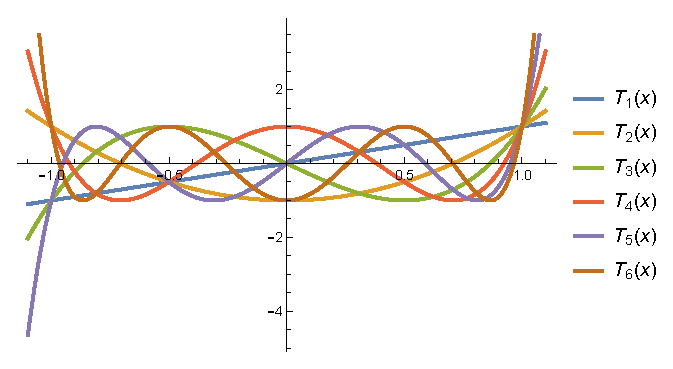
\includegraphics[scale=1]{Imagenes/Plot_Polinomios_Chebychev_01.eps}
    \caption{Primeros polinomios de Chebychev de primera clase.}
    \label{fig:figura_plot_chebychev_01}
\end{figure}
En general, los polinomios de Chebychev $T_{n}(x)$ satisfacen:
\begin{align*}
T_{n}(-x) = (-1)^{n} \, T_{n} (x)
\end{align*}
que se puede deducir fácilmente a partir de la ec. (\ref{eq:ecuacion_18_056}). También es fácil deducir los siguientes valores especiales:
\begin{align*}
T_{n} (1) &= 1 \\[0.5em]
T_{n} (-1) &= (-1)^{n} \\[0.5em]
T_{2n} (0) &= (-1)^{n} \\[0.5em]
T_{2n+1} (0) &= 0
\end{align*}
Los primeros polinomios de Chebychev de segunda clase se pueden obtener fácilmente, se presentan a continuación los primeros:
\begin{table}[H]
\centering
\fontsize{14}{14}\selectfont
\begin{tabular}{p{6cm} p{6cm}}
$U_{0}(x) = 1$ & $U_{1} = 2 \, x$ \\[0.5em]
$U_{2}(x) = 4 \, x^{2} - 1$ & $U_{3} = 8 \, x^{3} - 4 \, x$ \\[0.5em]
$U_{4}(x) = 16 \, x^{4} - 12 \, x^{2} + 1$ & $U_{5} = 32 \, x^{5} - 32 \, x^{3} + 6 \, x$ \\[0.5em]
\vdots & \vdots
\end{tabular}
\end{table}
Las funciones que representan a los polinomios de Chebychev de segunda clase se presentan en la figura (\ref{fig:figura_plot_chebychev_02}):
\begin{figure}[H]
    \centering
    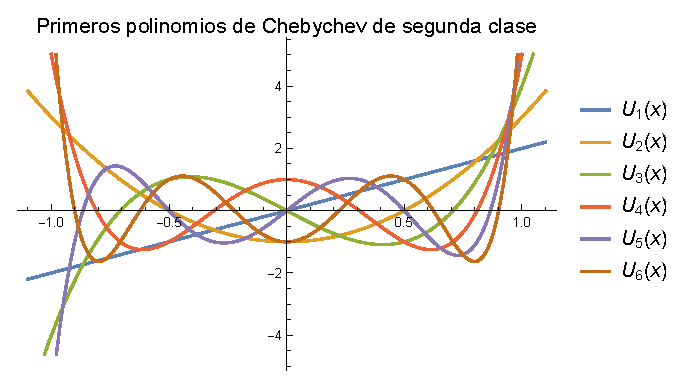
\includegraphics[scale=1]{Imagenes/Plot_Polinomios_Chebychev_02.eps}
    \caption{Primeros polinomios de Chebychev de segunda clase.}
    \label{fig:figura_plot_chebychev_02}
\end{figure}
Los polinomios de Chebychev $U_{n}(x)$ también satisfacen la propiedad:
\begin{align*}
U_{n} (-x) = (-1)^{n} \, U_{n} (x)
\end{align*}
la cual se puede deducir de las ecs. (\ref{eq:ecuacion_18_057}) y (\ref{eq:ecuacion_18_058}), y tiene, entre otros, los siguientes valores especiales:
\begin{align*}
U_{n} (1) &= n + 1 \\[0.5em]
U_{n} (-1) &= (-1)^{n} \, (n + 1) \\[0.5em]
U_{2n} (0) &= (-1)^{n} \\[0.5em]
U_{2n+1} (0) &= 0
\end{align*}

\section{Propiedades de los polinomios de Chebychev.}

Los polinomios de Chebyshev $T_{n} (x)$ y $U_{n} (x)$ tienen sus principales aplicaciones en el análisis numérico.
\par
Su uso para representar otras funciones en el rango $\abs{x} < 1$ juega un papel importante en la integración numérica; la cuadratura Gauss-Chebyshev es de particular relevancia para la evaluación precisa de integrales cuyos integrandos contienen factores del tipo $(1 - x)^{\pm 1/2}$.
\par
Por tanto, conviene destacar algunas de sus principales propiedades.
\subsection{Fórmula de Rodrigues.}
Los polinomios de Chebychev $T_{n}(x)$ y $U_{n}(x)$ se pueden expresar en términos de una fórmula de Rodrigues, de manera similar que las otras funciones especiales; se tiene que:
\begin{align*}
T_{n}(x) &= \left[ \dfrac{(-1)^{n} \, \sqrt{\pi} \, (1 - x^{2})^{1/2}}{2^{n} \, \left( n - \dfrac{1}{2} \right)!} \right] \, \dv[n]{x} (1 - x^{2})^{n-1/2} \\[0.5em]
U_{n}(x) &= \left[ \dfrac{(-1)^{n} \, \sqrt{\pi} \, (n+1)}{2^{n+1} \, \left( n - \dfrac{1}{2} \right)! (1 - x^{2})^{1/2}} \right] \, \dv[n]{x} (1 - x^{2})^{n+1/2}
\end{align*}

\subsection{Ortogonalidad mutua.}
La ecuación diferencial de Chebychev se puede ajustar a una del tipo Sturm-Liouville con $p = (1 - x^{2})^{1/2}$, $\lambda = n^{2}$ y $\rho = (1 - x^{2})^{-1/2}$, su intervalo natural es $[-1, 1]$.
\par
Como los polinomios de Chebychev de primera clase $T_{n}(x)$, son soluciones de la ecuación diferencial de Chebychev y son regulares en los puntos extremos $x = \pm 1$, deben de ser mutuamente ortogonales en este intervalo con respecto a la función de peso $\rho = (1 - x^{2})^{1/2}$, es decir:
\begin{align}
\int_{-1}^{1} T_{n}(x) \, T_{m}(x) \, (1 - x^{2})^{-1/2} \dd{x} = 0 \hspace{1.5cm} \mbox{si  } n \neq m
\label{ec:ecuacion_18_061}
\end{align}
La ortogonalización cuando $m = n$, es fácil de deducir haciendo la sustitución $x = \cos \theta$ y usando la ec. (\ref{eq:ecuacion_18_055}), de donde se obtiene el resultado:
\begin{align}
\int_{-1}^{1} T_{n} (x) \, T_{n} (x) (1 - x^{2})^{-1/2} \dd{x} = \begin{cases}
\pi & \mbox{para  } n = 0 \\[0.5em]
\dfrac{\pi}{2} & \mbox{para  } n = 1, 2, 3, \ldots
\end{cases}
\label{eq:ecuacion_18_062}
\end{align}
Para los polinomios de Chebychev de segunda clase $U_{n}(x)$, vemos que de la ec. (\ref{eq:ecuacion_18_058}):
\begin{align*}
(1 - x^{2})^{1/2} \, U_{n} (x) = V_{n+1} (x)
\end{align*}
satisface la ecuación diferencial de Chebychev (\ref{eq:ecuacion_18_054}) con $\nu = n + 1$. Por lo que la relación de ortogonalidad para los $U_{n}(x)$ se obtiene al reemplazar $T_{i}(x)$ por $V_{i+1} (x)$ en la ec. (\ref{ec:ecuacion_18_061}), obteniendo:
\begin{align*}
\int_{-1}^{1} U_{n}(x) \, U_{m}(x) \, (1 - x^{2})^{1/2} \dd{x} = 0 \hspace{1.5cm} \mbox{si  } n \neq m
\end{align*}
La correspondiente condición de normalización cuando $n = m$, se puede obtener al hacer nuevamente la sustitución $x  = \cos \theta$:
\begin{align*}
\int_{-1}^{1} U_{n}(x) \, U_{n}(x) \, (1 - x^{2})^{1/2} \dd{x} = \dfrac{\pi}{2}
\end{align*}

\subsection{Expansión de funciones.}
Dadas las condiciones de ortogonalización y normalización, permiten que cualquier función (razonable) pueda expandirse en el intervalo $\abs{x} < 1$ en una serie de la forma:
\begin{align*}
f(x) = \dfrac{a_{0}}{2} + \sum_{n=1}^{\infty} a_{n} \, T_{n} (x)
\end{align*}
en donde los coeficienes en la expresión están dados por:
\begin{align*}
a_{n} = \dfrac{2}{\pi} \int_{-1}^{1} f(x) \, T_{n} (x) \, (1 - x^{2})^{-1/2} \dd{x}
\end{align*}
Para los polinomios de Chebychev de segunda clase, también es posible expandir cualquier función razonable, en el intervalo $\abs{x} < 1$ en una serie de la forma:
\begin{align*}
f(x) = \sum_{n=0}^{\infty} a_{n} \, U_{n} (x)
\end{align*}
en donde los coeficientes $a_{n}$ están dados por:
\begin{align*}
a_{n} = \dfrac{2}{\pi} \int_{-1}^{1} f(x) \, U_{n}(x) \, 
\end{align*}

\subsection{Funciones generatrices.}

Las fuciones generatrices para los polinomios de Chebychev de primera y segunda clase, están dados respectivamente por las expresiones:
\begin{align}
G_{I} (x, h) &= \dfrac{1 - x \, h}{1 - 2 \, x \, h + h^{2}} = \sum_{n=0}^{\infty} T_{n} (x) \, h^{n} \label{eq:ecuacion_18_063} \\[0.5em]
G_{II} (x, h) &= \dfrac{1}{1 - 2 \, x \, h + h^{2}} = \sum_{n=0}^{\infty} U_{n} (x) \, h^{n} \label{eq:ecuacion_18_064}
\end{align}
Estas definiciones pueden probarse de manera similar a la utilizada para la función generadora de los polinomios de Legendre. Para los polinomios de Chebyshev, sin embargo, las funciones generadoras son de uso menos práctico, ya que la mayoría de los resultados útiles se pueden obtener más fácilmente aprovechando las formas trigonométricas (\ref{eq:ecuacion_18_055}), como se verá a continuación.

\subsection{Relaciones de recurrencia.}

Hay varias relaciones de recurrencia útiles para los polinomios de Chebychev $T_{n}(x)$ y $U_{n}(x)$, la mayoría de ellas se deducen fácilmente al hacer $x = \cos \theta$ y usando las ecs. (\ref{eq:ecuacion_18_055}) y (\ref{eq:ecuacion_18_058}), así tendremos:
\begin{align}
T_{n} (x) &= T_{n} (\cos \theta) = \cos n \theta \label{eq:ecuacion_18_065} \\[0.5em]
U_{n} (x) &= U_{n} (\cos \theta) = \dfrac{\sin (n + 1) \theta}{\sin \theta} \label{eq:ecuacion_18_066} 
\end{align}
Luego, se puede usar la fórmula estándar para las funciones trigonométricas para derivar una amplia variedad de relaciones de recurrencia. De particular utilidad son las identidades trigonométricas:
\begin{align}
\cos (n \pm 1)\theta &= \cos n \theta \, \cos \theta \mp \sin n \theta \, \sin \theta \label{eq:ecuacion_18_067} \\[0.5em]
\sin (n \pm 1)\theta &= \sin n \theta \, \cos \theta \pm \cos n \theta \, \sin \theta \label{eq:ecuacion_18_068}
\end{align}
Dos importantes relaciones de recurrencia son:
\begin{align}
T_{n+1} (x) - 2 \, x \, T_{n} (x) + T_{n-1} (x) &= 0 \label{eq:ecuacion_18_069} \\[0.5em]
U_{n+1} (x) - 2 \, x \, U_{n} (x) + U_{n-1} (x) &= 0 \label{eq:ecuacion_18_070}
\end{align}
Las relaciones de recurrencia (\ref{eq:ecuacion_18_069}) y (\ref{eq:ecuacion_18_070}) son extremadamente útiles en el cálculo práctico de polinomios de Chebyshev. Por ejemplo, dados los valores de $T_{0} (x)$ y $T_{1} (x)$ en algún punto $x$, el resultado dado por la ec. (\ref{eq:ecuacion_18_069}) puede usarse iterativamente para obtener el valor de cualquier $T_{n} (x)$ en ese punto; de manera similar, la ec. (\ref{eq:ecuacion_18_070}) puede usarse para calcular el valor de cualquier $U_{n} (x)$ en algún punto $x$, dados los valores de $U_{0} (x)$ y $U_{1} (x)$ en ese punto.
\par
Otras relaciones de recurrencia que satisfacen los polinomios de Chebyshev son:
\begin{align}
T_{n} (x) &= U_{n}(x) - x \, U_{n-1} (x) \label{eq:ecuacion_18_071} \\[0.5em]
(1 - x^{2}) \, U_{n} (x) &= x \, T_{n+1} (x) - T_{n+2} (x) \label{eq:ecuacion_18_072}
\end{align}
que establecen relaciones útiles entre los dos conjuntos de polinomios $T_{n} (x)$ y $U_{n} (x)$. La relación (\ref{eq:ecuacion_18_071}) se sigue inmediatamente de (\ref{eq:ecuacion_18_068}), mientras que la ec. (\ref{eq:ecuacion_18_072}) se sigue de la ec. (\ref{eq:ecuacion_18_067}), con $n$ reemplazado por $n + 1$, al observar que $\sin \theta = 1 - x^{2}$. Pueden obtenerse resultados útiles adicionales relacionados con los derivadas de los polinomios de Chebyshev a partir de las ecs. (\ref{eq:ecuacion_18_065}) y (\ref{eq:ecuacion_18_066}):
\begin{align*}
\ptilde{T}_{n} (x) &= n \, U_{n-1} (x) \\[0.5em]
(1 - x^{2}) \, \ptilde{U}_{n} (x) &= x \, U_{n} (x) - (n + 1) \, T_{n+1} (x)
\end{align*}
\end{document}